\documentclass[conference]{IEEEtran}
\IEEEoverridecommandlockouts
% The preceding line is only needed to identify funding in the first footnote. If that is unneeded, please comment it out.
\usepackage{cite}
\usepackage{amsmath,amssymb,amsfonts}
\usepackage{algorithmic}
\usepackage{graphicx}
\usepackage{textcomp}
\usepackage{xcolor}

\def\BibTeX{{\rm B\kern-.05em{\sc i\kern-.025em b}\kern-.08em
T\kern-.1667em\lower.7ex\hbox{E}\kern-.125emX}}
\begin{document}

\title{Experimental Bolus Sensor for Dairy Cattle\\
%\thanks{Identify applicable funding agency here. If none, delete this.}
}

\author{\IEEEauthorblockN{Gergely Vakulya}
\IEEEauthorblockA{\textit{Alba Regia Technical Faculty} \\
\textit{Óbuda University}\\
Székesfehérvár, Hungary \\
vakulya.gergely@amk.uni-obuda.hu}
\and
\IEEEauthorblockN{Éva Hajnal}
\IEEEauthorblockA{\textit{Alba Regia Technical Faculty} \\
\textit{Óbuda University}\\
Székesfehérvár, Hungary \\
hajnal.eva@amk.uni-obuda.hu}
\and
\IEEEauthorblockN{Péter Udvardy}
\IEEEauthorblockA{\textit{Alba Regia Technical Faculty} \\
\textit{Óbuda University}\\
Székesfehérvár, Hungary \\
udvardy.peter@amk.uni-obuda.hu}
}

\maketitle

\begin{abstract}
  A great challenge of today's humanity is to serve the intensively
  increasing demand for food, in an environmentally friendly manner.
  A promising way to address this problem is precision agriculture,
  based on extensive monitoring. In our research we focus on dairy
  cattle and rumen bolus sensors. This paper presents the preliminary
  results of an experimental bolus, equipped with accelerometer,
  shock sensor and temperature meter. During the measurement a bolus sensor was settled into the rumen of the examined cattle and a video recording was saved at the same time. The recorded data set was examined from movement activity, heart rate, body temperature baseline aspects.
\end{abstract}

\begin{IEEEkeywords}
  dairy cattle, bolus, accelerometer, jerk
\end{IEEEkeywords}

\section{Introduction}

A great challenge of today’s humanity is to serve the intensively increasing
demand for food, in an environmentally friendly manner. A promising way to
address this problem is precision agriculture, based on extensive monitoring \cite{berckmans2014, hokofarm2019}.
From the point of view of animal welfare, continuous monitoring of animals is
very important, which makes it possible to monitor the health status of animals
and to optimize animal husbandry to maximize milk yield \cite{john2016, aidin2019} based on economic
considerations. Rumen boluses play a very important role in this process. This
area has been intensively investigated in the last twenty, but especially in
the last few years. Rumen boluses were used first for identification
\cite{RUIZGARCIA201142, hanton1974}, then for the delivery of medicines and active
ingredients, and finally for the monitoring of animals \cite{nagl2003}, typically for short
periods. The first such sensors were used to monitor rumen pH \cite{neubauer2018}. In recent years,
advances in sensor technology, battery technology, and data transmission
technologies have made it possible to develop sensors that can be used for many
years, essentially for the entire lifetime of the animal, and the cost allows
for all-animal use. In the case of such a sensor, there is a need to obtain as
much information about the animals as possible and later process them in a big
data system \cite{Cabrera2021}. In this paper, a preliminary experiment of such a sensor is
presented, emphasizing the extraction of as much information as possible from
the measured data. The research question is whether the designed sensor is
suitable for continuous measurement and data transmission and what additional
derived characteristics can be obtained from the obtained primary data, which
can be used later for the benefit of animal husbandry. The second chapter of
the article deals with the description of the experimental site and conditions.
The 3rd chapter deals with the configuration of the device and the description
of the experiment, as well as the description of the data processing.
Chapter 4 discusses the actual data processing steps and the obtained results,
as well as the evaluation of the results. Chapter 5 concludes the paper and
presents future directions for development.


%\begin{table}[htbp]
%\caption{Table Type Styles}
%\begin{center}
%\begin{tabular}{|c|c|c|c|}
%\hline
%\textbf{Table}&\multicolumn{3}{|c|}{\textbf{Table Column Head}} \\
%\cline{2-4} 
%\textbf{Head} & \textbf{\textit{Table column subhead}}& \textbf{\textit{Subhead}}& \textbf{\textit{Subhead}} \\
%\hline
%copy& More table copy$^{\mathrm{a}}$& &  \\
%\hline
%\multicolumn{4}{l}{$^{\mathrm{a}}$Sample of a Table footnote.}
%\end{tabular}
%\label{tab1}
%\end{center}
%\end{table}

\section{Measurement environment}

The experiment was carried out on a large-scale dairy farm at ‘Agárdi Farm Ltd’ in the Central-Transdanubian region of Hungary. The farm was formed on the base of the former ‘Agárdi state farm’ after the political changes in the early 90’s and has 5850 hectares of arable land. The farm deals with plant production, animal husbandry and game management. More than 300 hectares of the arable land is irrigated. The forage for the animal husbandry are produced locally.
The farm has a herd of over 900 lactating Holstein cows. From the 28th day before calving, dry cows are housed in a pre-calving group pen (measuring 35 m × 20 m), which include 50 to 60 animals and is bedded with deep straw. Before calving, cows are fed a prepartum total mixed ration (TMR) ad libitum containing a dietary forage to concentrate ratio of 81.7:18.3 on a dry mater (DM) basis. The chemical composition of the bovine milk is highly depending on the forage quality and feeding method \cite{aidin2019}.

Calvings take place in the prepartum group pen or, if continuous supervision or obstetrical assistance is required at calving, in a separate maternity pen. Within 1 hour after calving the dam is being milked, and 3.8 litres fresh colostrum is provided to the new-born calves by nipple bottle. If the colostrum of the dam is low quality or insufficient, calves receive frozen colostrum.

During the first 5 days in milk, cows are housed in postpartum pens, each including 4 animals and are milked twice daily at 4 AM and 2 PM in a four-stall herringbone milking parlor operated with DeLaval Control Valve bucket milking machines (DeLaval International AB, Tumba, Sweden).

After 5 days in milk, cows are introduced to the fresh lactation group and milked three times daily at 6 AM, 12 AM and 6 PM in a 2 × 28-stall parallel Bosmark milking parlor (Bosmark Kft., Biatorbágy, Hungary).

\section{Measurement setup}

\subsection{Bolus sensor}

Design of the bolus is constrained by several factors. As these type
of devices are getting more and more standard, special applicators are
exist to inject them into the rumen. The physical dimensions are therefore
limited by the applicator. The desired form factor is a cylinder with
diameter of 40 mm and length of 140 mm.

The material of the bolus should resist the environment inside the rumen,
i.e. the moisture, temperature, motion and pH. The cover should protect
the sensitive electronics inside sensor. The POM-C technical plastic was
chosen as the material, which can be easily machined on a lathe and provides
the required strength and sealing.

A more or less fixed orientation of the bolus would ease the signal
processing of the accelerometer. To provide some defined orientation
in at least one axis the weight distribution of the bolus is designed
to be asymmetrical, the battery being one one end and a low density
material on the other side. The electronics are placed in between these two.

\begin{figure}[htbp]
  \centerline{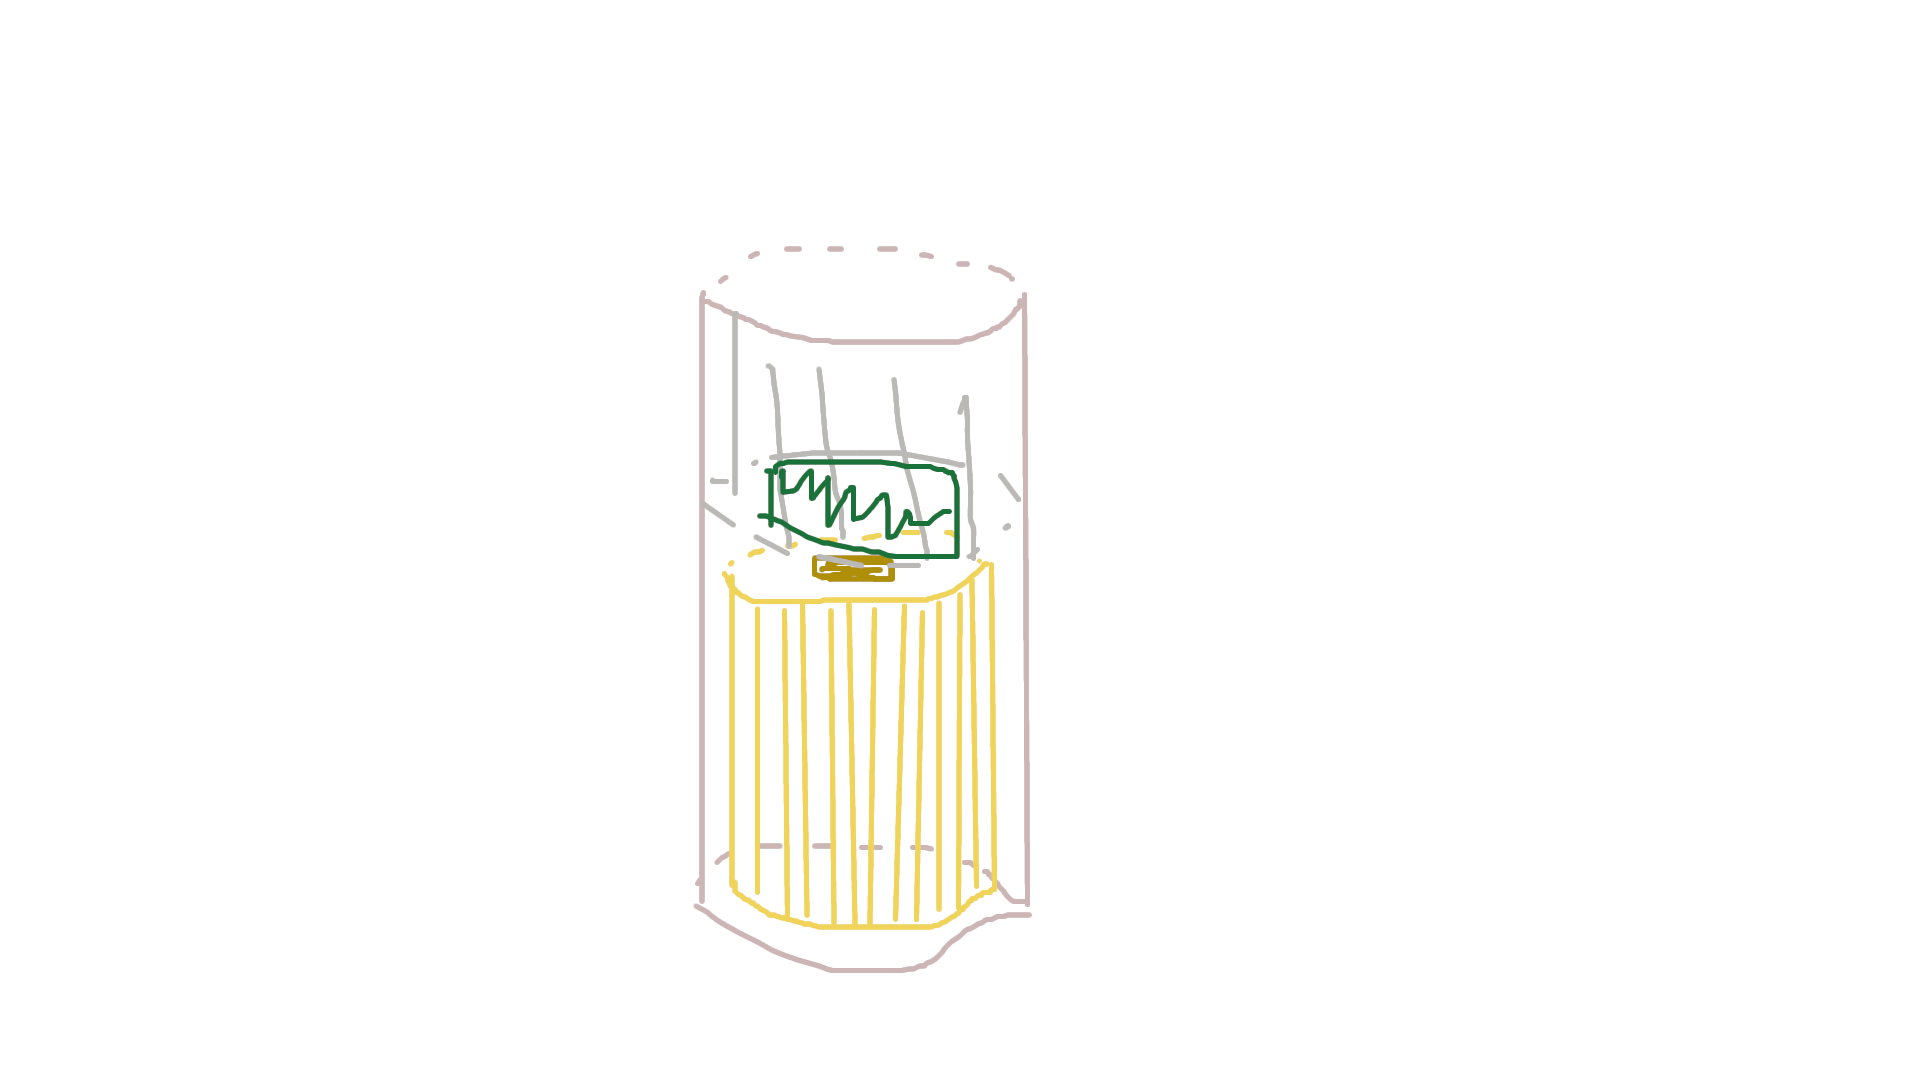
\includegraphics[width=0.48\textwidth]{fig/bolus-physical-layout.png}}
  \caption{The physical layout of the bolus.}
  \label{bolus-physical-layout}
\end{figure}

The physical layout of the bolus is shown in Fig. \ref{bolus-physical-layout}.
The power source of the unit is a non-rechargeable D type Lithium battery,
which provides 3.7 V and 18 Ah capacity and most of the mass. The
microcontroller on the circuit board is a TODO, which controls the
sensors and the radio.

The accelerometer is a TODO, which has 16 bit resolution on 3 axes and
set to 25 Hz sample rate. This gives a good balance between the available
bandwidth and the data processing possibilities. This modality is extended
with an additional shock detector. This sensor acts as a simple contact switch,
which activates when an abrupt motion event happens. The microcontroller
counts the number of detections in every second.

The third sensor is a digital temperature meter (TODO type), which gives
a precision of 0.1 \textcelsius.

Since the body of the cattle gives significant attenuation of RF signals
the radio chip, the communication frequency and modulation was chosen very
carefully. The body of the animals tends to give more attenuation on higher
frequencies (especially 2.4 GHz seems to be a bad decesion), but on the
other hand lower frequencies require larger antennas to the same gain.
Another compromise is present between the data bandwidth and the link budget.
In this design the TODO digital radio was chosen. It operates in the 169 MHz
band and has a raw bandwith of TODO kbps. In this frequency a
$\lambda / 4 \approx 42 cm$ would be ideal, which clearly cannot be fit
inside the bolus, therefore a much smaller, approx. 6 cm wire antenna
was used.

\begin{figure}[htbp]
  \centerline{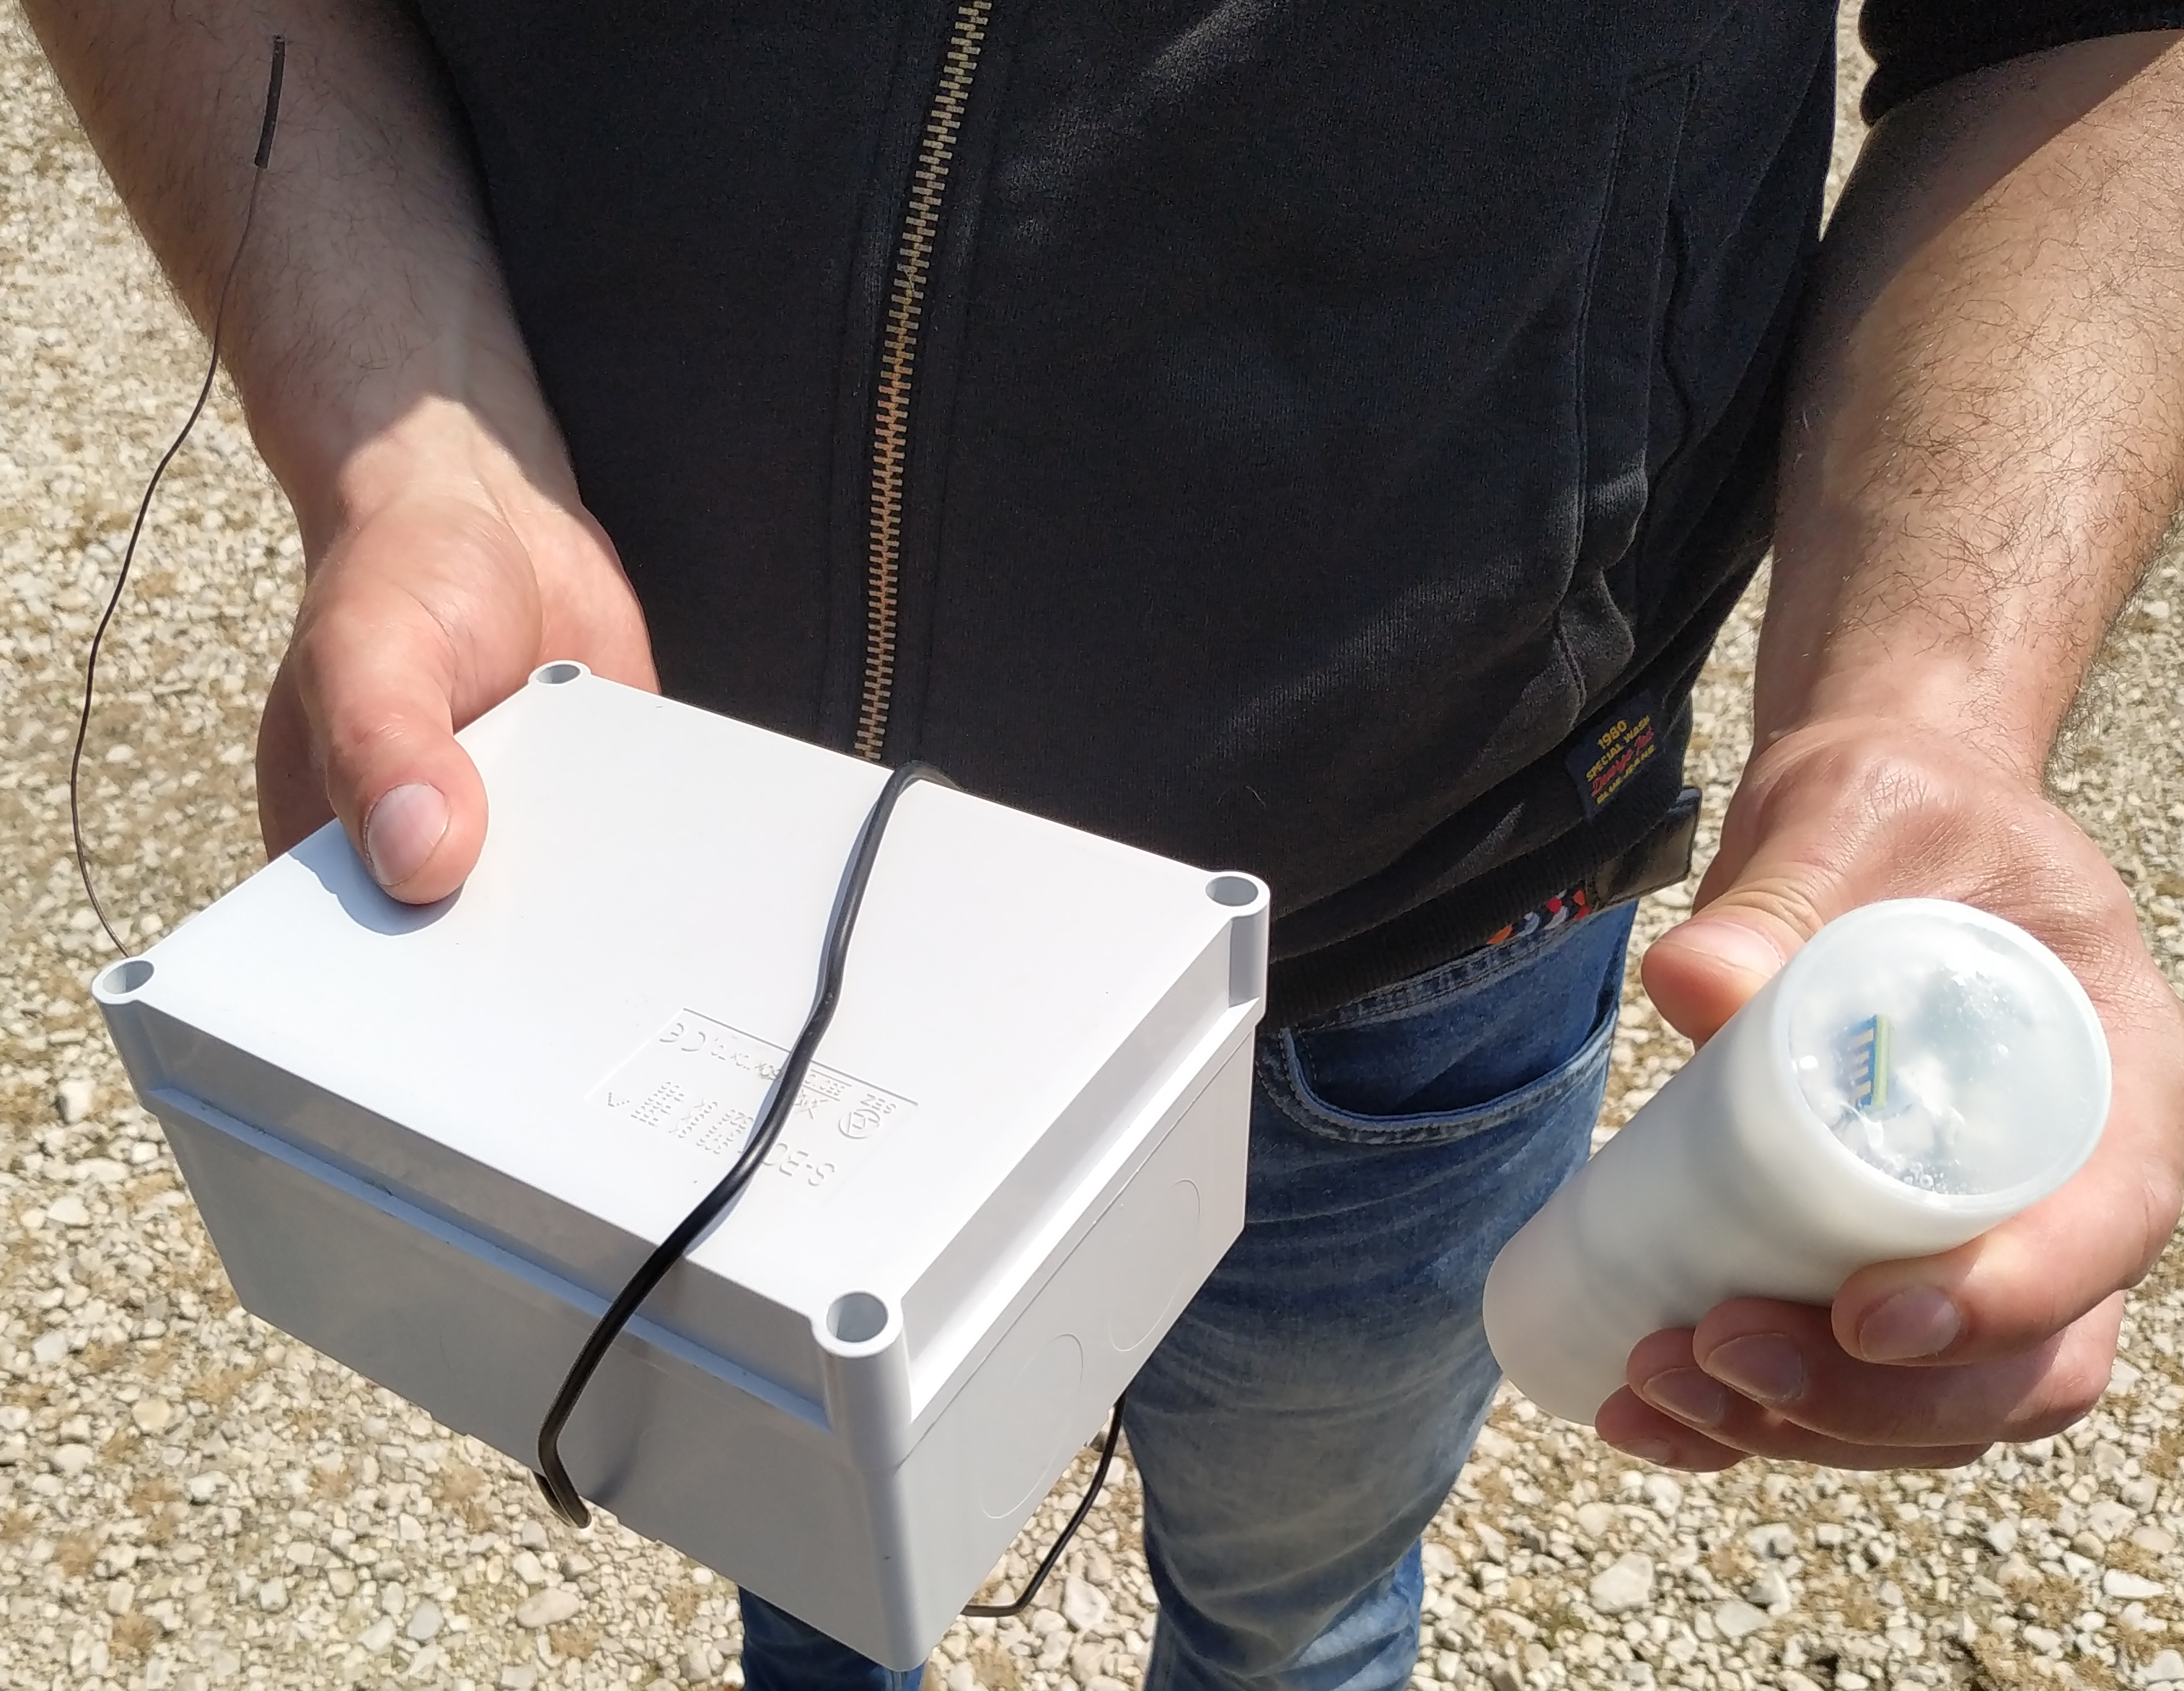
\includegraphics[width=0.48\textwidth]{fig/bolus_gw_photo.jpg}}
  \caption{The bolus (right side) and the gateway (left side).}
  \label{bolus-gw-photo}
\end{figure}

\subsection{Gateways}

The gateways (see Fig. \ref{bolus-gw-photo}) are responsible for receiving
the signals from the bolus and
storing the collected data. The gateway is based on a Raspberry Pi 2 model B.
This single board computer has an ARM processor running at 700 MHz, 512 MB of
RAM and an SD card for the operating system and data storage. Since the
Raspberry Pi does not have a battery backed realtime clock the date and
time has to be set on startup to ensure correct timestamps to the
measurements.

The RF packets are received by a similar radio transceiver to the one inside the
bolus. The radio and the SBC are connected through a serial-to-USB converter.

The gateway sends an acknowledgment to every received packet. If the bolus
does not receive the ACK it tries to transmit the packet at most twice more.
This mechanism procects against short interferences. Although the bolus does
not store unsuccessfully delivered packets, therefore those measurements are
lost.

\subsection{Data format}

The received data is logged in CSV (Comma Separated Values) format. This gives
flexibility to analyze collected data in a vide variety of programming languages
(for example Python, R, or C) or in Excel. The data collection software records
each received packet in a row. A single packet contains one second of data.
An example line from the data record is shown in Fig. \ref{csv-sample}. The first
value is a standard Unix timestamp represented as a floating point number to provide
higher resolution. The next field is the serial number of the packet. This helps to
detect missing packets. Then 25 triplets of integers follow, which belong to the
25 measurements taken by the acceletometer with the 3 axes. It is followed by
a counter value from the shock sensor. The last number is the RSSI (Received
Signal Strength Indicator), in dBm.
of shock events.

\begin{figure}[htbp]
\begin{verbatim}
1651672339.971273,95810,-15344,-3024,3132,
-15656,-3120,3336,-15652,-3108,3840,-15308,
-3404,4076,-15336,-3432,3924,-15148,-3796,
3900,-15020,-3772,3896,-15032,-3756,4008,
-15212,-3632,3888,-15396,-3704,3572,-15568,
-3528,3712,-15716,-3340,3904,-15492,-3288,
3868,-15364,-3212,3736,-15432,-3184,3528,
-15564,-3204,3392,-15816,-3472,3424,-15984,
-3400,3736,-15976,-3052,3980,-15812,-2976,
4064,-15800,-3112,4140,-15652,-2960,4112,
-15636,-3124,4076,-15484,-3136,3968,-15360,
-3128,3904,42.75,0,-80.5
\end{verbatim}
\caption{A sample line from the recorded data}
\label{csv-sample}
\end{figure}


\subsection{Injecting the bolus}

\begin{figure}[htbp]
  \centerline{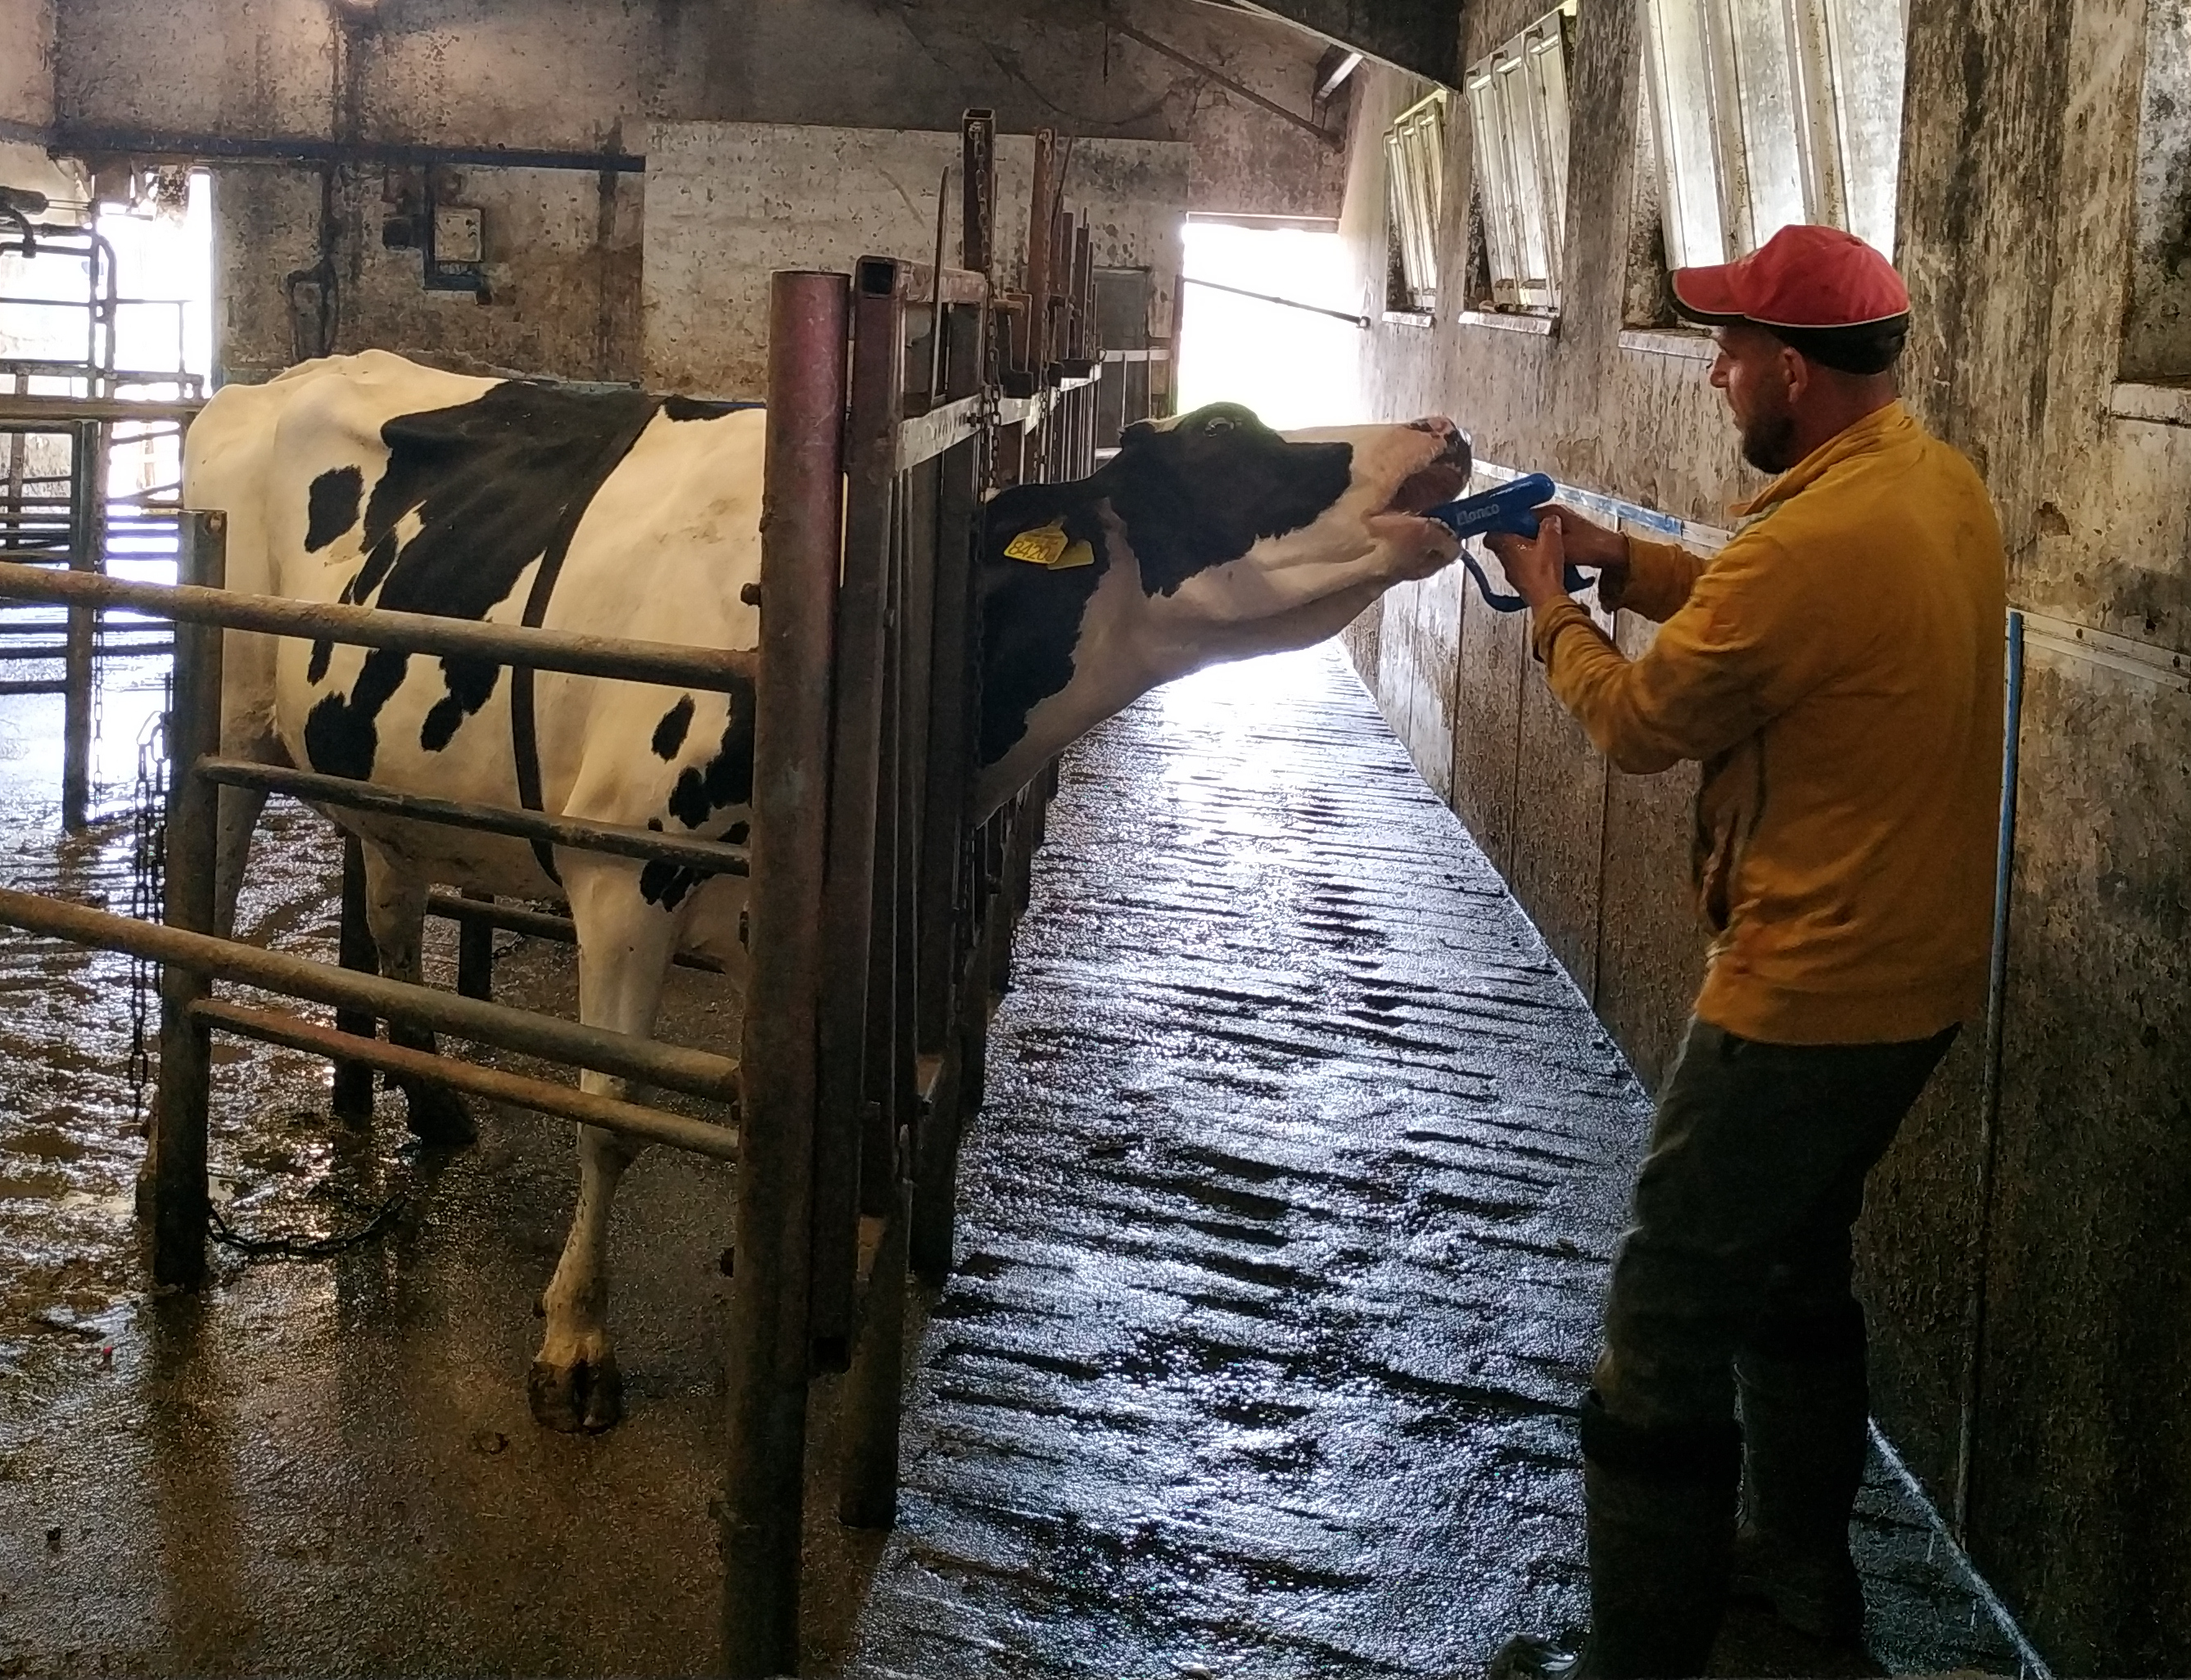
\includegraphics[width=0.48\textwidth]{fig/bolus_application.jpg}}
  \caption{Injecting the bolus with the applicator.}
  \label{bolus-injecting}
\end{figure}


\section{Results}

\subsection{Analyzing the radio communication}

Radio communication is one of the most important function of the bolus. It heavily
impacts the quality of the measurements 

\subsection{Validating of self-orienatation}

First the self-orienting behavior of the bolus sensor was tested outside the
rumen in water. The bolus was placed horizontally in the middle of the bucket,
then it was released. The bolus reached a vertical orientation in about 2 seconds,
as can be seen in Fig. \ref{self-orientation-experiment}.

\begin{figure}[htbp]
  \centerline{
    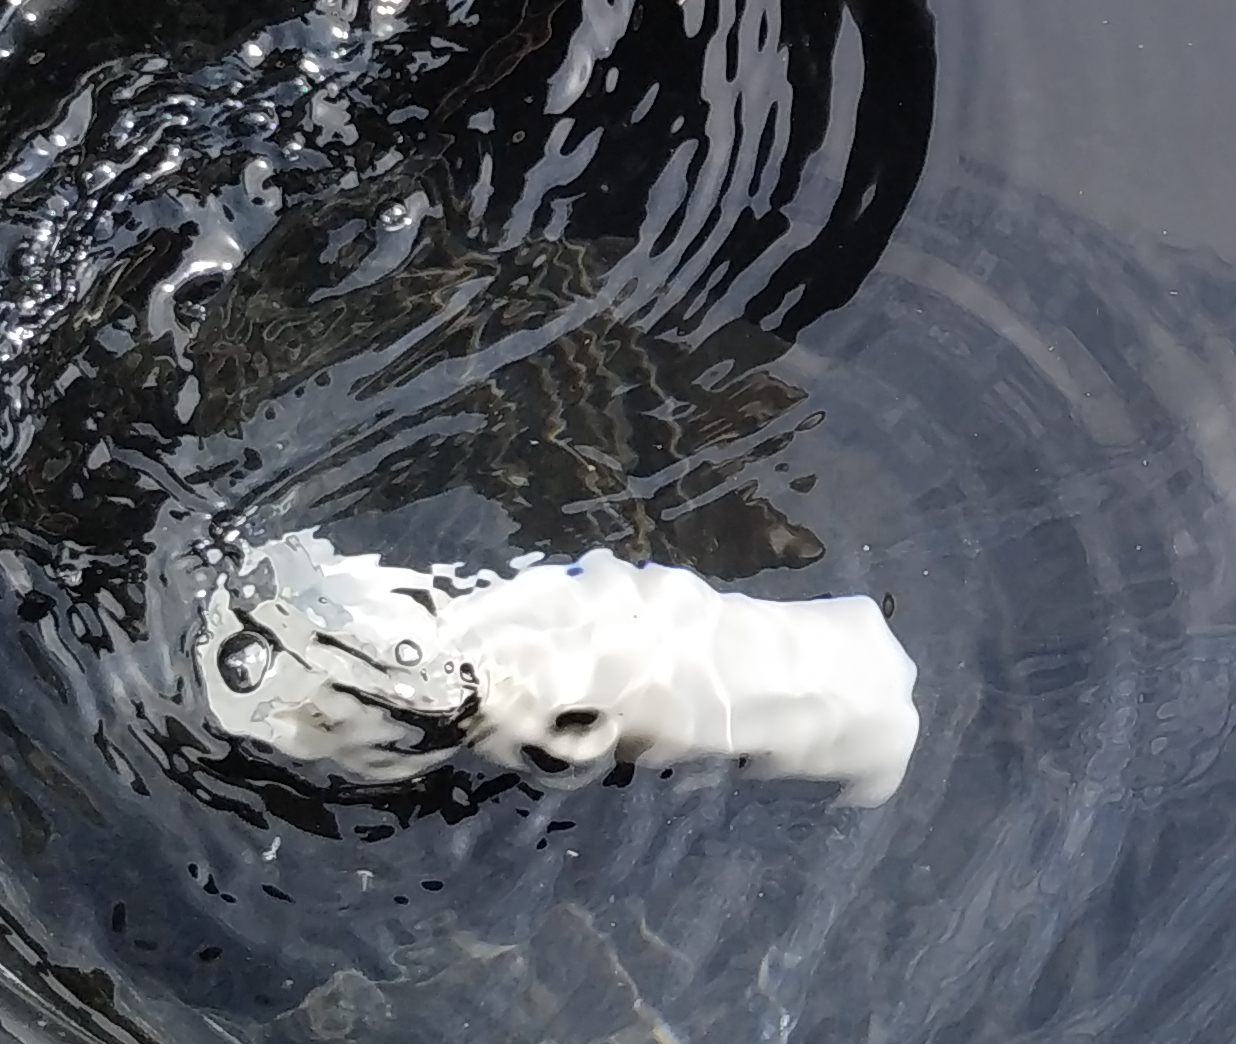
\includegraphics[width=0.15\textwidth]{fig/kfj_1.png}
    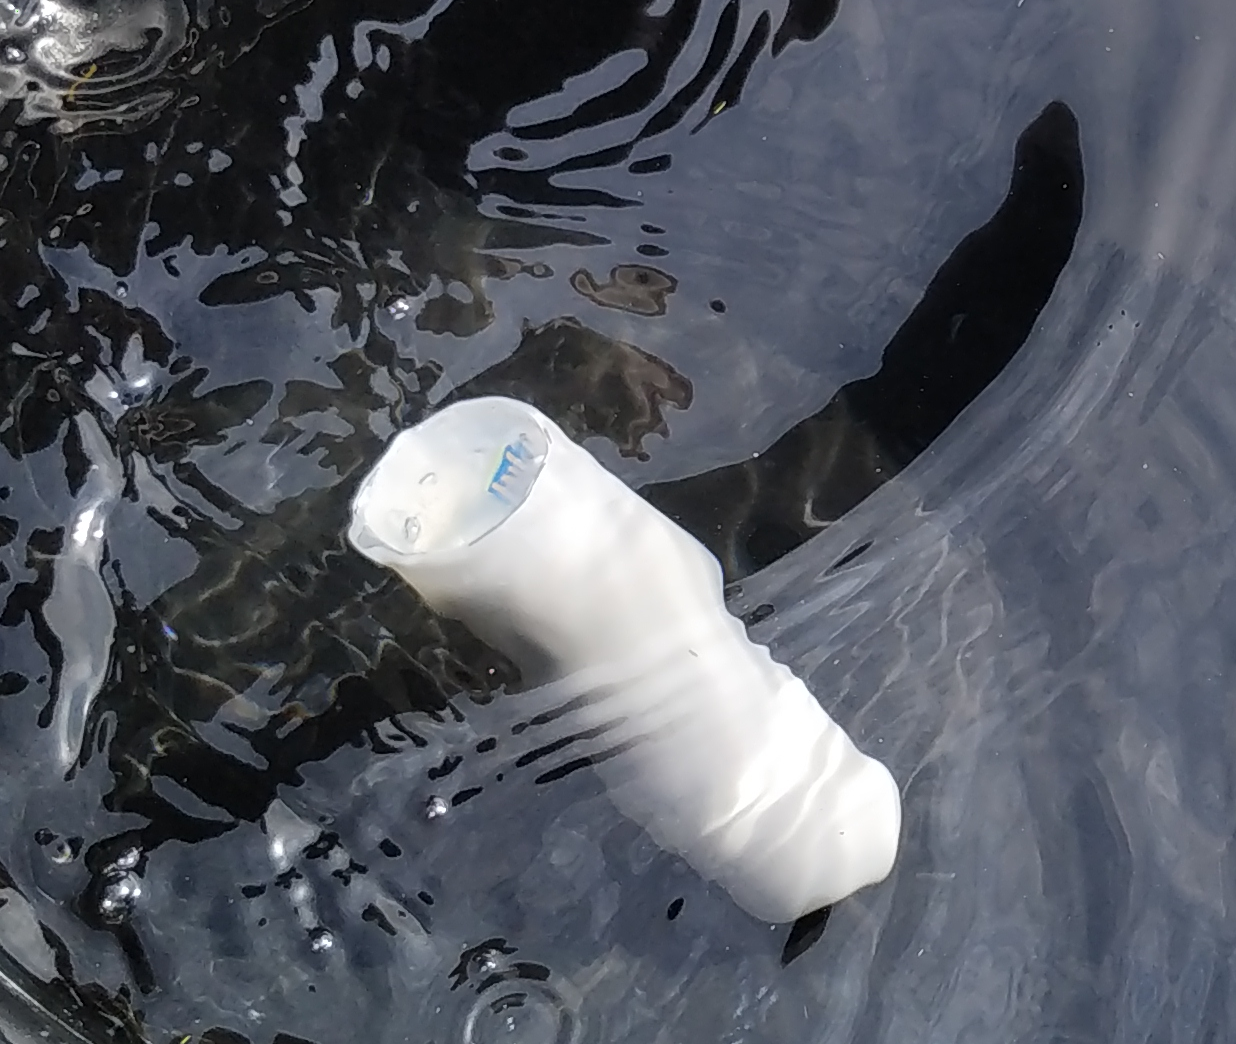
\includegraphics[width=0.15\textwidth]{fig/kfj_2.png}
    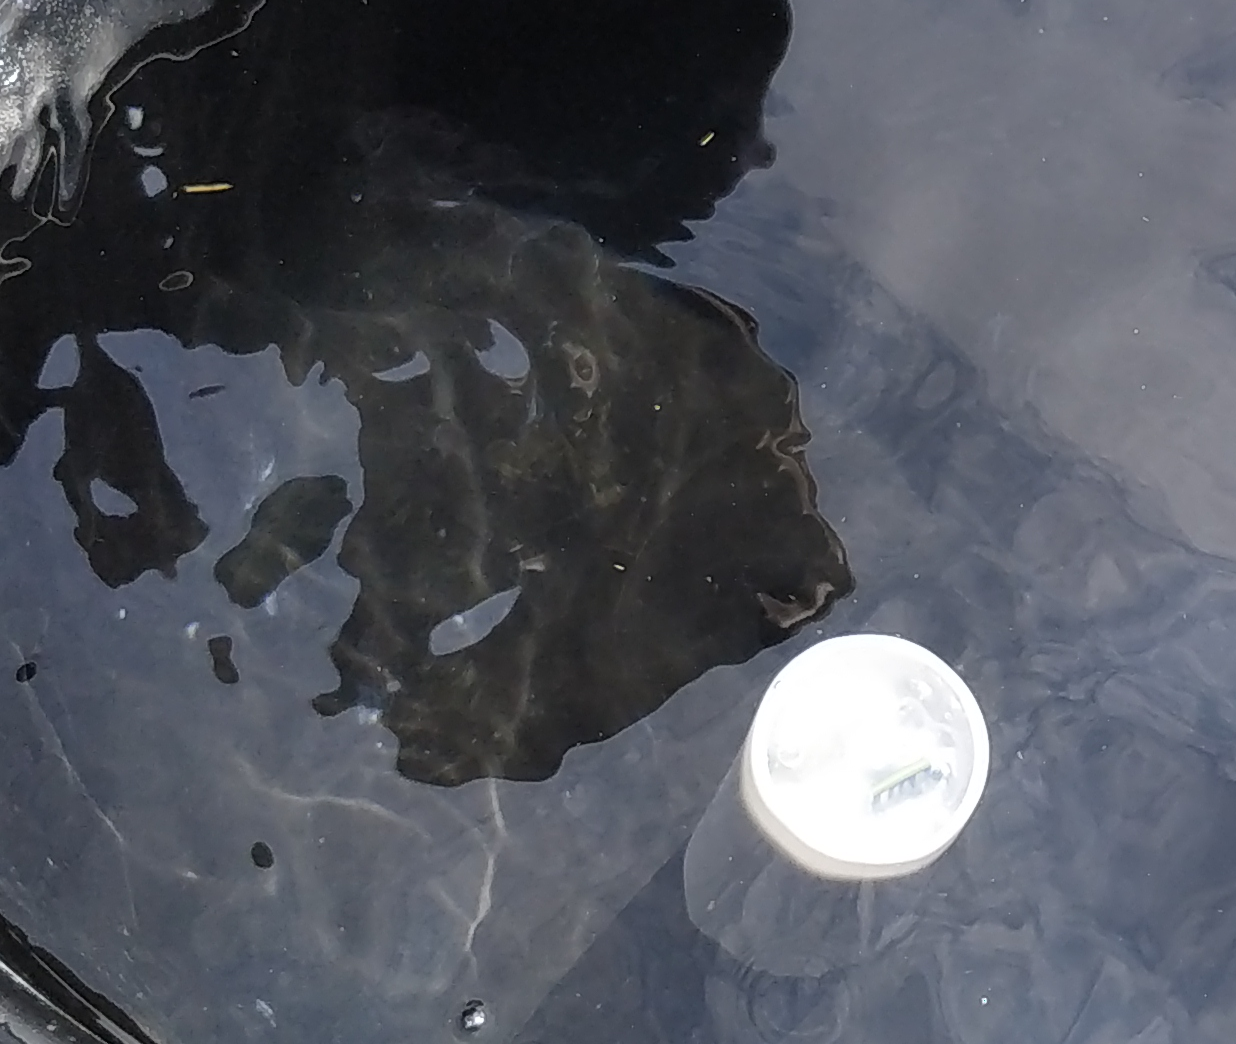
\includegraphics[width=0.15\textwidth]{fig/kfj_3.png}
  }
  \caption{Experiment of the self-orientation of the bolus sensor. The
  bolus is placed in a horizontal position in water (left side), then takes
  an upright position (middle, then right side).}
  \label{self-orientation-experiment}
\end{figure}

To validate the self-orientation behavior of the bolus inside the rumen,
a time interval was
selected, when the animal significantly changed their position (lays down,
in our case). As the \emph{z} axis is parallel with the longitudinal axis
of the bolus, we expect near 1 G of acceleration in this direction, when
the animal either standing or lying. We also expect a transient phase in
between these two.

To validate this phenomenon the samples collected along the \emph{z} axis
were processed. First a $2^{nd}$ order Butterworth lowpass filter was
applied to the data with corner frequency of 5 mHz. This very low
frequency suppresses most of the higher frequency noises and provides
a smooth output. From the filtered acceleration data the vertical
angle of the bolus was calculated with an inverse sinus function.
The resulting graph can be seen in Fig. \ref{auto-orientation}.

\begin{figure}[htbp]
\centerline{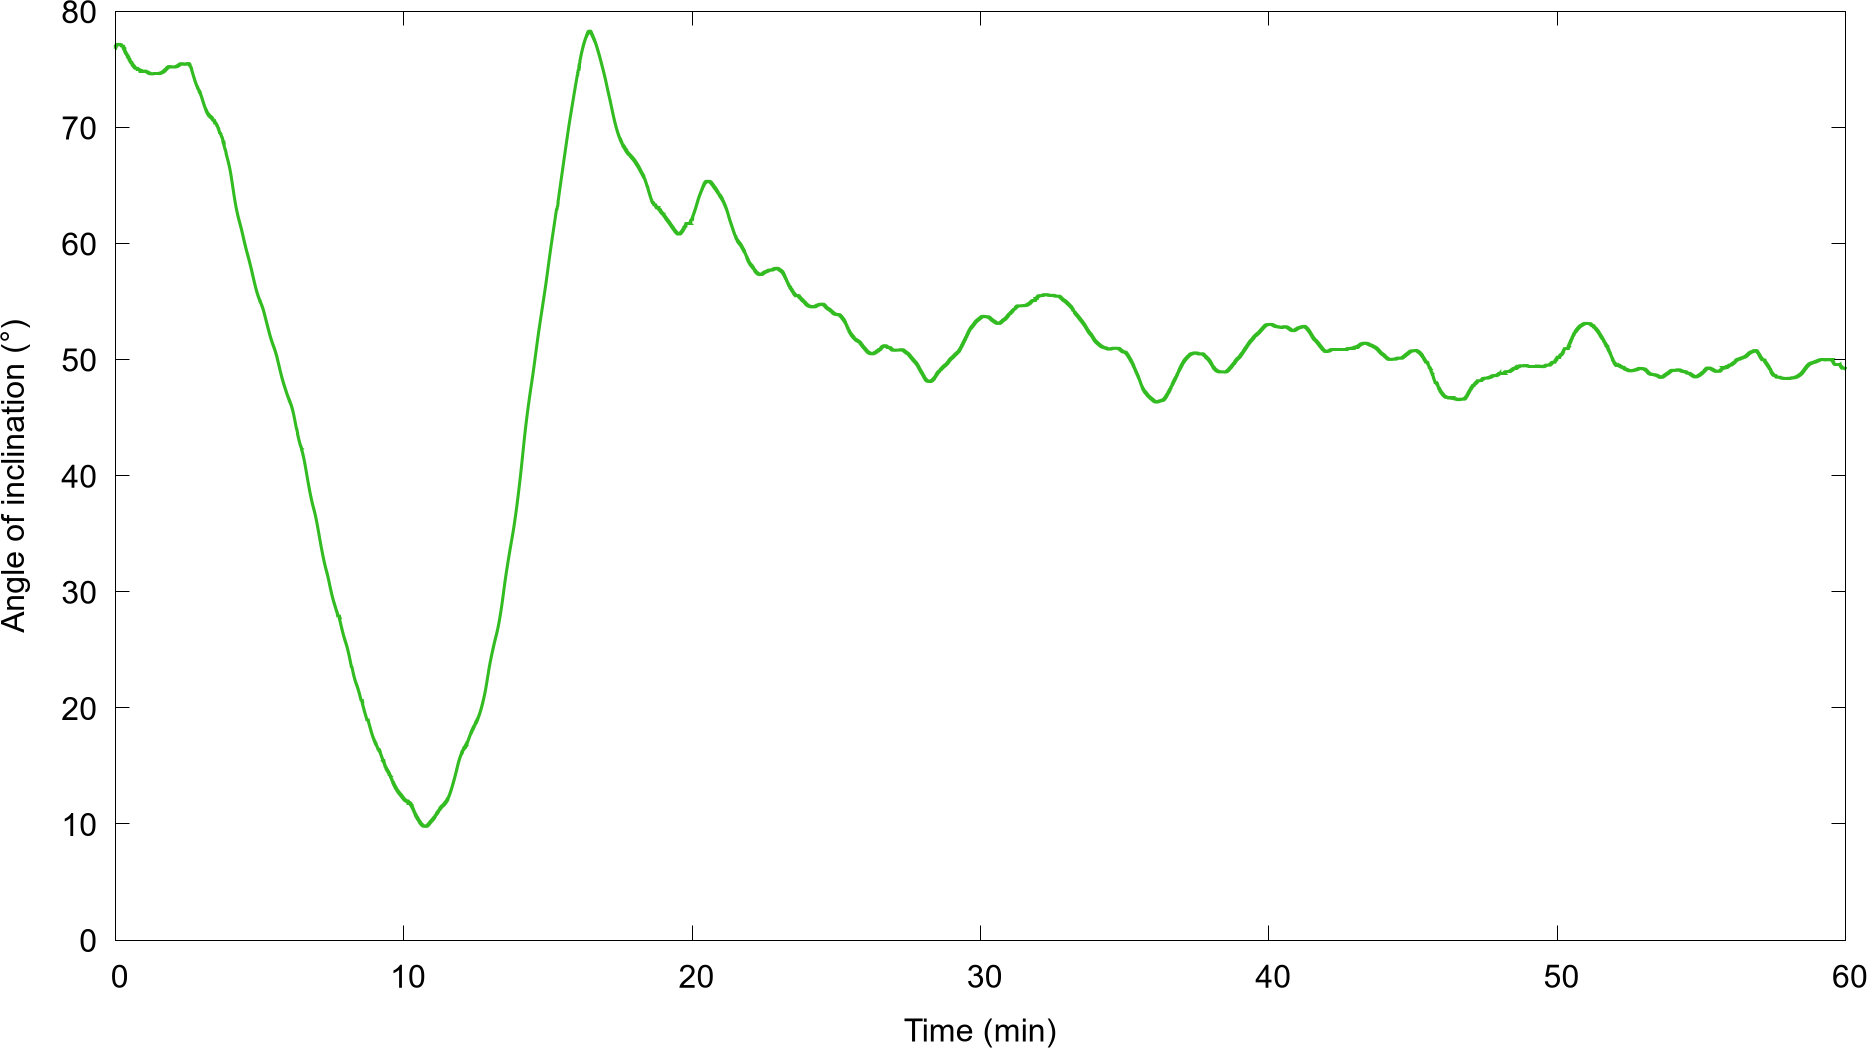
\includegraphics[width=0.48\textwidth]{fig/auto-orientation.png}}
  \caption{Changing of the orientation of the bolus}
\label{auto-orientation}
\end{figure}

In the first 3 minutes the graph shows a near vertical state (about
75\textdegree). Then the animal probably made a significant movement,
when the bolus reached a near horizontal position (about 10\textdegree)
in 8 minutes and got back to a near vertical orientation (about 80
\textdegree) again in 8 minutes. Int the remaining time the bolus
has a more or less stable orientation between 50\textdegree and
80\textdegree.

According to this experiment the bolus tends to get a vertical, or a near
vertical orientation, but this procedure is several orders of magnitude
slower inside the rumen than in water.
\subsection{Activity analysis}
The general movement activity is an important feature of cattle and its monitoring  is essential. However the activity measurements can be a subject of another paper, in this article only the stepping activity  is presented. Monitoring the quantity of walking gives information about the general health of the animal and both the quantity and the detailed feature can be special indicators of the lameness. The stepping activity is shown on Fig.\ref{walking}. This chart shows the special doulbe peaked curve of the walking with the appropriate ampltude and 1-2s period length. The preprocessing of data was the calculation of the resultant acceleration, followed by filtering with lowpass Butterworth filter at 2.5Hz, and the calculation of the jerk of this processed resultant and finished with lowpass Butterworth filtering at 2.5 Hz and visualization.

\begin{figure}[htbp]
\centerline{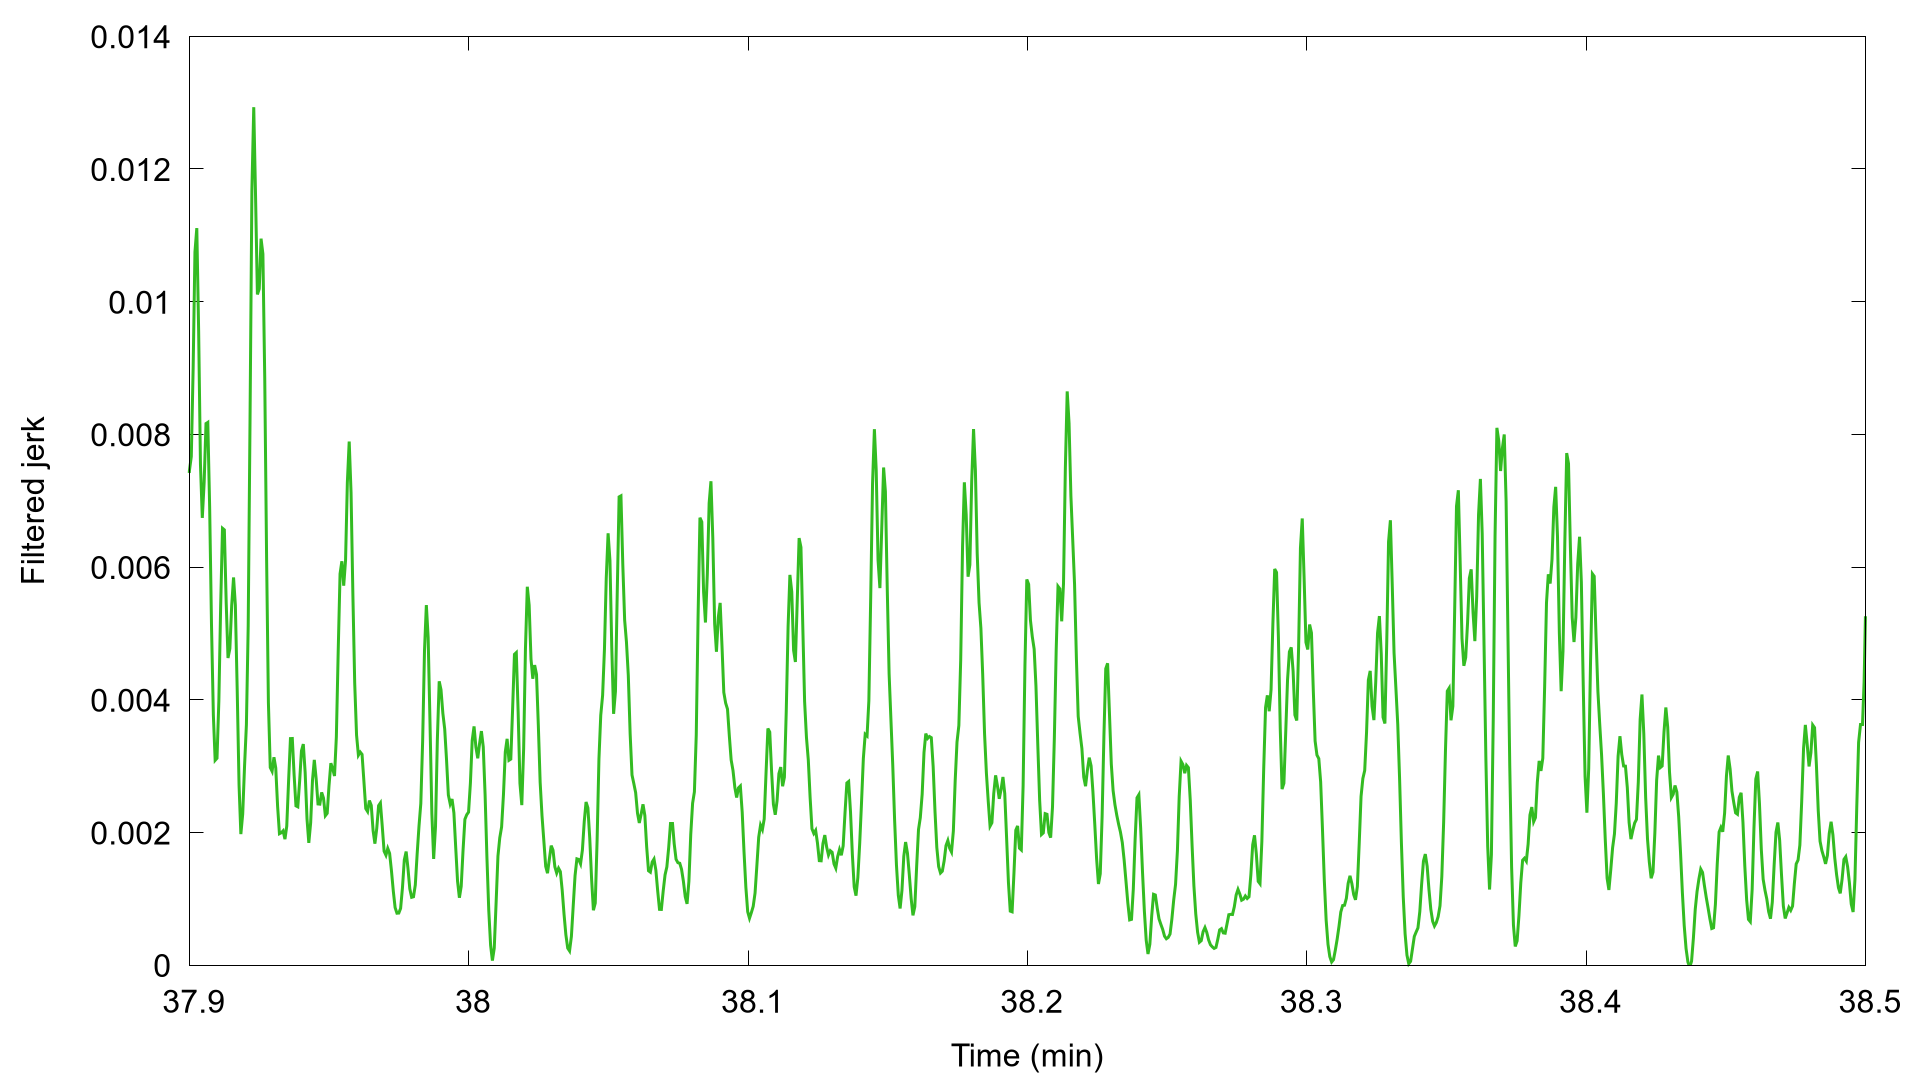
\includegraphics[width=0.48\textwidth]{fig/plot_ker.png}}
  \caption{Sample data from the accelerometer preprocessed for detecting movement activity, visualized
  in time domain.}
\label{walking}
\end{figure}


\subsection{Rumination}

Rumination is a very important activity of cattles of which monitoring is essential. Rumination is a periodic movements of the rumen with large amplitude (near 0.01-0.02G) and larger period length. The typical period is between 40 and 80 second. For detecting rumination, according to the literature a preprocessing calculation was executed, namely the jerk of each axis and the resultant of the jerks were calculated followed with the rolling variance in 1.5s long window and finally a rolling average with 8s long window. The resulted time series must show periodic accelerations with the mentioned attributes. Fig.\ref{rumination} shows a mixed signal with periodic sign of rumination in the first 5 minutes and after that a nonperiodic activity.
\begin{figure}[htbp]
\centerline{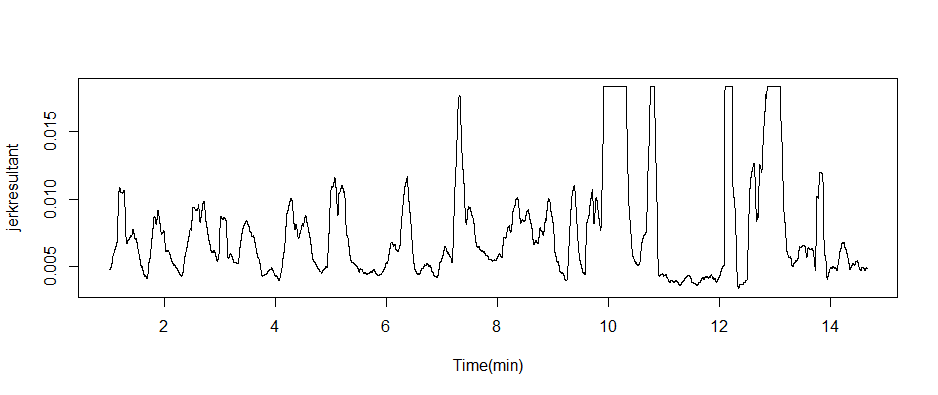
\includegraphics[width=0.48\textwidth]{fig/rumination.png}}
  \caption{Sample data from the accelerometer preprocessed for detecting rumination, visualized
  in time domain.}
\label{rumination}
\end{figure}

\subsection{Heart rate and respiration analysis}

Weak signals caused by the heartbeats and the respiration can only analyzed
in calm periods. Based on the video recording and the standard deviation
of the acceleration data a calm periods were selected with length of 36 sec.
Data were preprocessed for analysis, namely the outliers were replaced with mean value and a moving average was calculated with 8 data width window. The resulted time series is in Fig.\ref{heart-time-domain}  shows the selected signal in time domain.

\begin{figure}[htbp]
\centerline{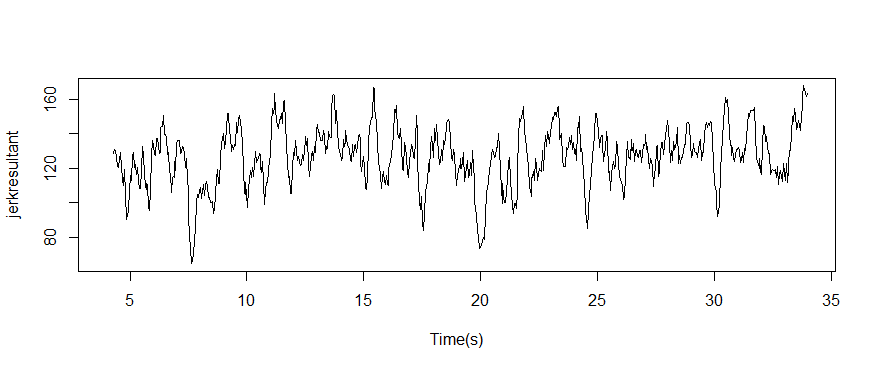
\includegraphics[width=0.48\textwidth]{fig/ts_heart.png}}
  \caption{Sample data from the accelerometer during a calm period, visualized
  in time domain.}
\label{heart-time-domain}
\end{figure}

Heart rate analysis was taken with Wavelet-Morlet analysis with 8s long data periods. 
The results were plotted for visual analysis. The heart rate first and second harmonic were visible on 90 percentage of randomly chosen data samples and heart rate safely identified on 70 percentage of the samples. The heart rate is visible between 0.5 and 1 s period length (Fig.\ref{heart-wavelet}). The signals of respiration are visible between 2s and 4s period length. It is important to note that the amplitude of the heart signal is near 0.003G but the amplitude of the respiration is weaker, because the movements of the respiration are more calm and "smooth". Furthermore the background physical phenomenon is different in accelerometer measurements to the traditional ECG measurements. This later measurement based on detecting electric signals of the heart but this former measurement based on detecting the acceleration data generated by heart muscles movements.   According to this the respiration is visible only in 50-60 percentage of the randomly choosen data samples.

\begin{figure}[htbp]
\centerline{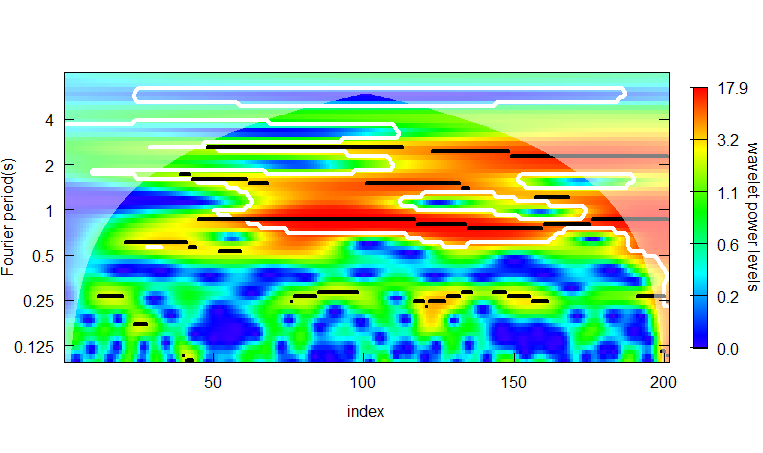
\includegraphics[width=0.48\textwidth]{fig/Wavelet.png}}
  \caption{Sample data visualized after wavelet transformation.}
\label{heart-wavelet}
\end{figure}

\subsection{Analysis of temperature meter data}

\section{Summary}

\section*{Acknowledgment}

“This research was funded by NKFI Hungary, grant number 2020-1.1.2-PIACI-KFI-2020-00109”. We would like to thank to Levente Kovács MATE Hungary for his advices.

\bibliographystyle{IEEEtran}
\bibliography{IEEEabrv,references}

\end{document}
